\subsection{Cosmic Radiation Methods}
\label{sec:Rad-Methods}

\begin{figure}[H]
	\begin{center}
	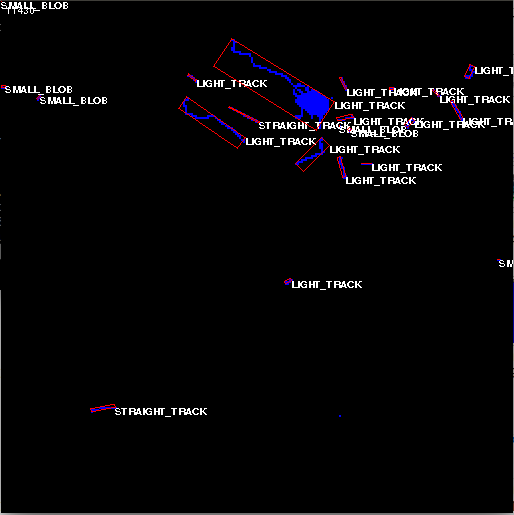
\includegraphics[width=0.6\textwidth]{figures/clustering.png}
	\caption{Bounding boxes calculated for a frame of flight data.}
	\label{clusterframe}
	\end{center}
\end{figure}

The output format of TimePIX devices provides a great deal of flexibility in terms of data analysis. The data can provide both a simple absorbed dose from ionizing radiation as well as insight into more detailed dosimetric endpoints like dose equivalent. Additionally a clustering procedure can be performed to analyze individual particle interactions in the detector based on their morphological properties.

 Since energy deposition can be determined on a per pixel basis, absorbed energy is calculated via a simple summation across all pixels in a frame of data after applying a standard calibration procedure \cite{mpjakubek}. With knowledge of the mass of the detector volume you can then calculate a dose by dividing the deposited energy by the detector mass. Thus a simple dose in silicon is calculated as

\[D_{Si} = \frac{E}{M_{d}}\]

To analyze the data on a per track basis first, a clustering procedure has to be performed to separate the data in a frame into individual tracks. This can be accomplished by applying a simple algorithm used in image processing called Flood-Fill; whereby contiguous nonzero pixels are recursively filled and grouped together into clusters. Then, after calculating a minimum area bounding box and linear least squares fit a track length is calculated by determining where the least square fit line intersects with the bounding box. Additionally, an azimuth angle can be determined relative to the detector orientation and a density can be calculated by dividing the number of pixels in a cluster by the area of the bounding box. A simple visual example of these calculations is shown in Figure \ref{track_analysis} and a visualization of the bounding boxes calculated for a frame of data is shown in Figure \ref{clusterframe}

\begin{figure}[H]
	\begin{center}
	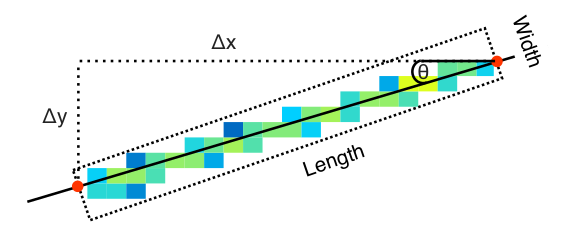
\includegraphics[width=0.8\textwidth]{figures/density.png}
	\caption{Track parameter calculation.\cite{stuartthesis}}
	\label{track_analysis}
	\end{center}
\end{figure}

Given the track length calculated from the fit line and the bounding box, a three-dimensional track through the detector by using simple trigonometry. Given the sensor thickness $T$ and the projected track length $L_{p}$ the length of the track through the detector $L$ can be calculated by

\[L = \sqrt{L_{p}^{2} + T^{2}} \]

With a true track length calculated one can then calculate the linear energy transfer ($LET$) of a track by dividing the total energy deposited in a cluster $E$ by the track length $L$.

\[LET_{Si} = \frac{E}{L}\]

Another standard technique used when analyzing TimePIX data is sorting clusters in the data based on their morphological characteristics. After clustering, additional processing is applied to calculate individual track parameters. These parameters can then be placed into a simple sorting algorithm that assigns them labels based roughly on their characteristics. The idea behind this morphological analysis is that information regarding the origin of the particle that made the track can be elucidated on the principle that similar types of particles will create similar shaped tracks in the detector. Based on a tracks density, pixel count, inner pixel count and ratio between the bounding box's length and width a track is sorted as either a small blob, medium blob, heavy blob, light track, straight track or heavy track. The specifics of the algorithm are defined in Figure \ref{stuart_algo}.

\begin{figure}[H]
	\begin{center}
	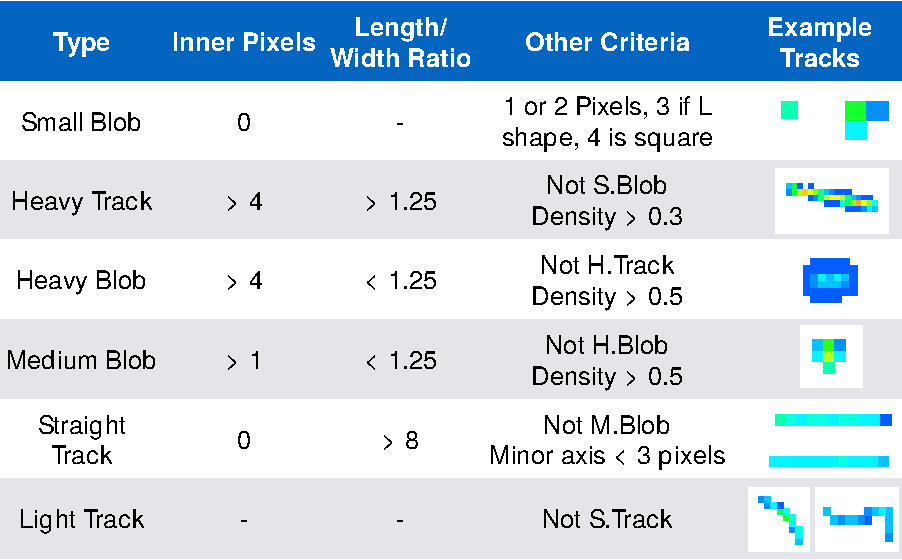
\includegraphics[width=0.65\textwidth]{figures/stuartgraphic.pdf}
	\caption{Track morphology algorithm.\cite{stuartalgo}}
	\label{stuart_algo}
	\end{center}
\end{figure}

While the track morphology does not provide a hard and fast classification a rough idea of the origin of a track in a mixed radiation field can be determined. Possible origins of track morphology are shown in \ref{track_morphology}.

\begin{figure}[H]
	\begin{center}
	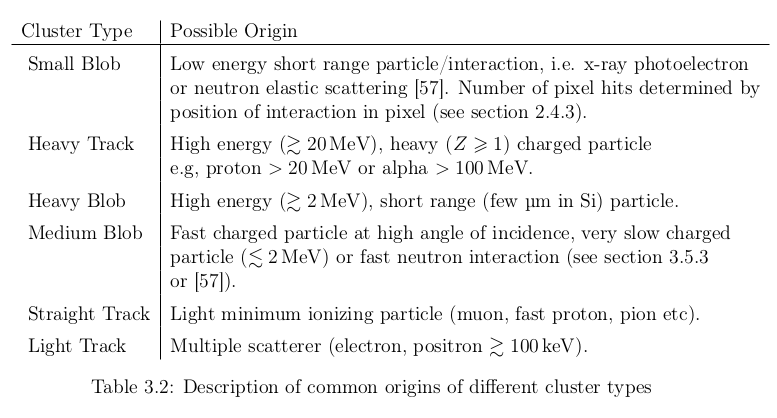
\includegraphics[width=0.8\textwidth]{figures/cluster_types.png}
	\caption{Possible physical origins of cluster morphology.\cite{stuartthesis}}
	\label{track_morphology}
	\end{center}
\end{figure}
